\section{Methodology}
\label{sec:methodology}

\subsection{Threat model}
We consider the following adversaries.
\begin{description}
	\item[Network-level adversary] An adversary that monitors at least
		one autonomous system, e.g., ISP, VPS provider, government.
	\item[Relay-level adversary] An adversary that runs at least one Tor relay.
	\item[DNS provider] An adversary that operates the DNS resolver used
		by exit relays, e.g., Google.
\end{description}

\begin{table}[t]
	\centering
	\begin{tabular}{ccc}
	\textbf{Type} & \textbf{Number of ASs} & \textbf{Percentage} \\
	\hline
	DNS & 369 & 70.4\% \\
	Web & 351 & 67.0\% \\
	DNS $\setminus$ Web & 173 & 33.0\% \\
	Web $\setminus$ DNS & 155 & 29.6\% \\
	DNS $\cap$ Web & 196 & 37.4\% \\
	DNS $\cup$ Web & 524 & 100\% \\
	\end{tabular}
	\caption{The set relations between unique traversed ASs for DNS and unique
	traversed ASs for Web.}
	\label{tab:traversed-ass}
\end{table}

\subsection{Exposure at the Exit side}
\begin{itemize}
	\item Rented VPS from OVH, representative for exit relay.
	\item Ran ddptr to Alexa top 1,000 sites.
	\item In total, traversed 30,872 ASs for DNS and 10,707 ASs for web,
		including duplicates.
	\item Eliminating duplicates, we traversed 369 unique DNS ASs and 351 unique
		web ASs.
	\item Among the 369 unique DNS ASes, 173 (46.9\%) were \emph{only} traversed
		for DNS, and not for web.
	\item Among the 351 unique web ASes, 155 (44.2\%) were \emph{only} traversed
		for web, and not for DNS.
	\item 196 ASes were part of both web and DNS ASes.
\end{itemize}

\subsection{Exposure at the Guard side}
\begin{itemize}
	\item Bad guards
	\item recognise dns requests by traffic analysis on the wire.  probably
		difficult because of optimistic data?  can we do more than just timing?
	\item can flow watermarking help?  see houmansadr's
		work~\cite{Houmansadr2011a}
\end{itemize}

\subsection{What resolvers do exits use?}
Figure~\ref{fig:dnsenum} shows how we can identify an exit relay's DNS resolver.
Over each exit relay, we resolve a unique domain \texttt{PREFIX.tor.nymity.ch}
for which we control the authoritative DNS server.  As a result, we can learn
the IP address of all resolvers that ask for a domain in
\texttt{*.tor.nymity.ch}.

\begin{figure}[t]
	\centering
	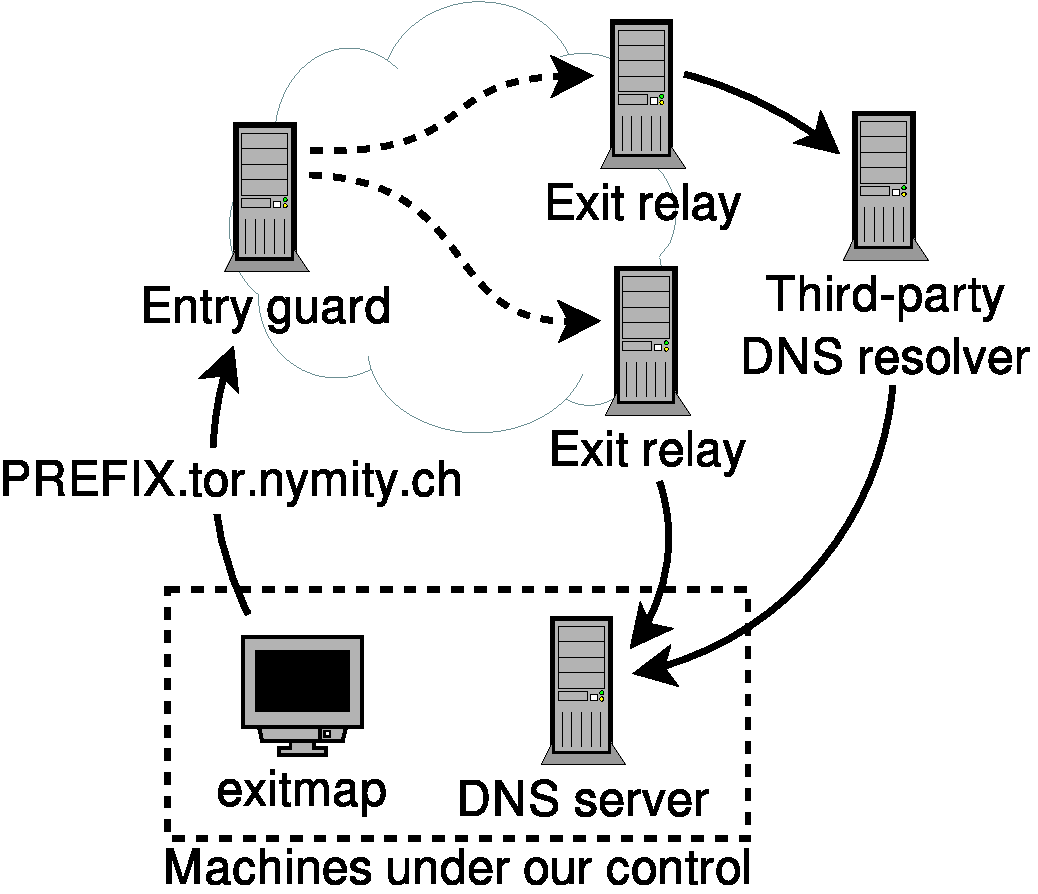
\includegraphics[width=0.8\linewidth]{figures/dns-resolver-enumeration.pdf}
	\caption{Our method to identify the DNS resolver of exit relays.  We resolve
	unique domain names under our control over each exit relay.  We then extract
	the IP address of all resolvers that contacts our DNS server, and map them
	to the respective exit relay.}
	\label{fig:dnsenum}
\end{figure}

An exit relay can either run its own resolver (see the bottom relay in
Fig.~\ref{fig:dnsenum}), or use a third-party resolver such as the one provided
by its ISP (see the top relay in Fig.~\ref{fig:dnsenum}).  If an exit relay runs
its own resolver, we expect to receive a DNS request from the exit relay's IP
address, but if an exit relay uses a third-party resolver, we expect to receive
a request from an unrelated IP address.

We can map DNS requests to exit relays because we encode the relay's 160-bit
unique fingerprint in \texttt{PREFIX}.  We also encode a 40-bit random value in
\texttt{PREFIX} make sure that our requests are not cached anywhere.  As a
result, we send DNS requests of the form
\texttt{FINGERPRINT.RAND.tor.nymity.ch}.

We used the tool exitmap~\cite{Winter2014b} to resolve our domain over all exit
relays.  For performance and reliability, we used only two-hop circuits,
consisting of a static guard relay under our control, and the exit relay.

We ran this experiment from Sep 2015 to Jan 2016, six times a day.

\begin{table}[t]
	\centering
	\begin{tabular}{rcc}
	\textbf{Pct.} & \textbf{Organization} & \textbf{Country} \\
	\hline
21.6 & Google & US \\ % -> 21.56 bw pct.
13.1 & Local resolver & --- \\ % -> 14.14 bw pct.
6.5 & OpenDNS & US \\ % -> 6.46 bw pct.
6.5 & OVH & FR \\ % -> 6.46 bw pct.
2.7 & S.A.S. & FR \\ % -> 2.65 bw pct.
2.5 & NFOrce Entertainment & NL \\ % -> 2.47 bw pct.
2.1 & UK2 & GB \\ % -> 2.07 bw pct.
2.0 & Iomart & GB \\ %  -> 1.96 bw pct.
1.9 & CYBERDYNE & LR \\ % -> 1.90 bw pct.
1.7 & DFRI & SE \\ % -> 1.74 bw pct.
% 1.7 & Level 3 Communications & US \\ % -> 1.72 bw pct.

% 	306 & 33.4\% & Google & US \\
% 	62 & 6.8\% & OVH SAS & FR \\
% 	26 & 2.8\% & OpenDNS & US \\
% 	23 & 2.5\% & Hetzner Online & DE \\
% 	18 & 2.0\% & S.A.S. & FR \\
% 	17 & 1.9\% & Hurricane Electric & US \\
% 	14 & 1.5\% & LeaseWeb Netherlands & NL \\
% 	12 & 1.3\% & Level 3 Communications & US \\
% 	8 & 0.9\% & Iomart & GB \\
% 	7 & 0.8\% & PlusServer & DE \\
% 	\hline
% 	71 & 7.7\% & Local resolver & \\
	\end{tabular}
	\caption{The top ten resolvers used by all exit relays by capacity on Jan 1,
	2016.  More than 20\% of all exit bandwidth at the time used Google's DNS
	server.  13.1\% of exit bandwidth is resolved by local DNS resolvers.}
	\label{tab:dns-resolvers}
\end{table}

\begin{figure}[t]
	\centering
	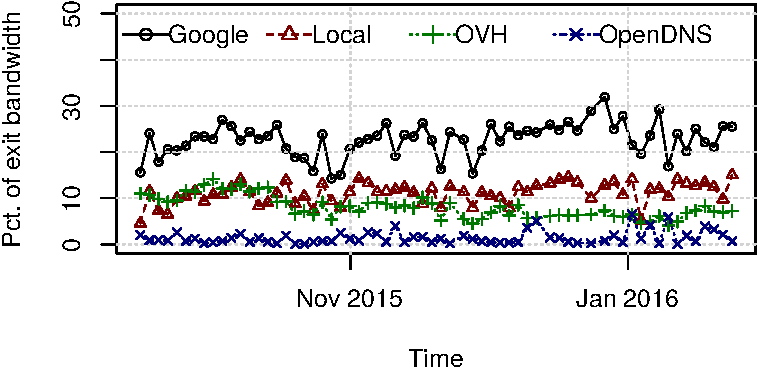
\includegraphics[width=\linewidth]{figures/exit-resolvers.pdf}
	\caption{The amount of the most popular DNS resolvers of exit relays over
	time, weighted by bandwidth.  Google's DNS server is by far the most popular
	resolver of exit relays, followed by a local resolver, OVH, and OpenDNS.}
	\label{fig:exit-resolvers}
\end{figure}


\subsection{Internet map}
\begin{itemize}
	\item Where do we get our AS and IXP graph from?
	\item Johnson et al.~\cite[\S 5.2]{Johnson2013a} used RouteViews and the CAIDA IPv4
		Routed /24 AS Links Dataset, resulting in 44,605 ASs connected by
		305,381 links.
\end{itemize}

\subsection{Traceroute dataset}
\label{sec:traceroute-dataset}
\begin{itemize}
	\item Find machines that are topologically close to DNS resolvers
		used by exit relays.
	\begin{itemize}
		\item RIPE Atlas probes.
		\item Virtual private systems.
		\item PlanetLab nodes.
		\item Ask exit operators to run traceroutes for us.
	\end{itemize}
	\item Run traceroutes to DNS servers to determine path coverage.
	\item Determine ``AS inflation factor.''
\end{itemize}

\subsection{DNS root dataset}
\label{sec:dns-root-dataset}
\begin{itemize}
	\item Learn what kind of domains are resolved by exit relays to learn where
		we should traceroute to.
	\item Minimize risks.
	\begin{itemize}
		\item Get rid of timestamps if at all possible, otherwise the dataset
			could be used to deanonymize people after publishing it.  Nick W.
			said that these could be useful to learn about caching, though.
	\end{itemize}
\end{itemize}

\subsection{DNS packet sizes at entry guard}
\begin{itemize}
	\item Send many DNS requests over entry guard.
	\item Capture them on the wire and look at them.
	\item What's the best way to filter out the noise?
\end{itemize}

\subsection{Practical attacks}
We leverage the following building blocks:
\begin{itemize}
	\item Traffic analysis done on an entry guard.  Can DNS requests be isolated
		reliably?
	\item Access to DNS root, .com, and .net.
	\item Ability to use DNS resolver's cache as an oracle.
	\item Ability to enumerate what resolver's an exit relay uses.
	\item Resolvers using EDNS.
	\item Users in country X are likely to resolve domains of country X.
\end{itemize}
